\documentclass[../../../main.tex]{subfiles}

\begin{document}

\subsubsection{pedestrian method}

\begin{center} 
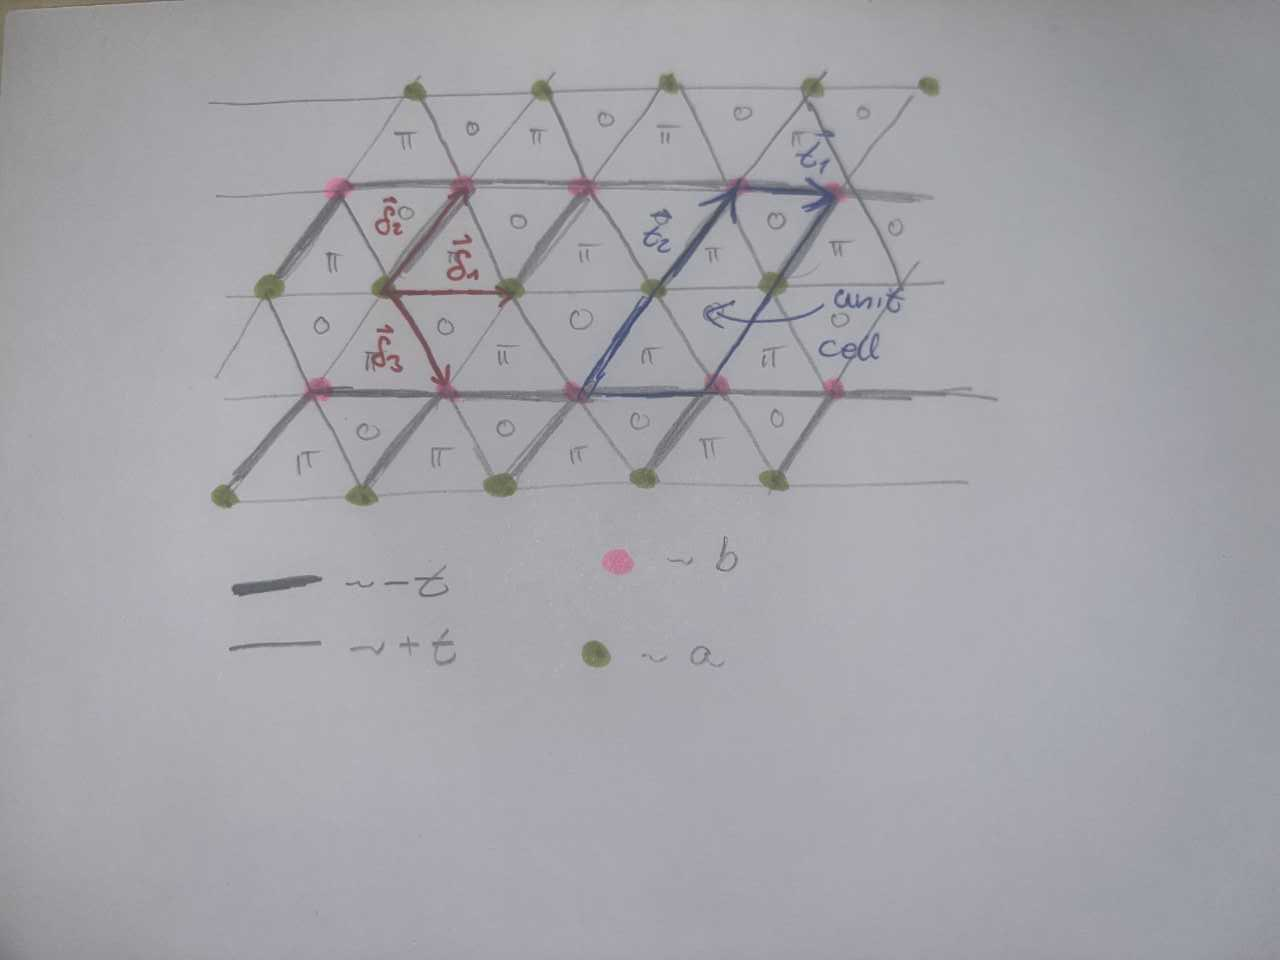
\includegraphics[width = \textwidth]{lattice-pi-0-flux-state.jpeg}
\end{center}

The system is a triangular bravais lattice with a two-atomic basis. The primitve translations are 

\begin{equation}
	\vec{a}_1=
	\begin{pmatrix}
		1 \\
		0
	\end{pmatrix}, \quad
	\vec{a}_2=
	\begin{pmatrix}
		1 \\
		\sqrt{3}
	\end{pmatrix}
\end{equation}

Hence, two types of lattice sites exist, a and b (see sketch). Also $\chi_{ij}$, and thereby $t_{ij}$ can change sign (see sketch). The Hamiltonian is

\begin{equation}
	H = \frac12\sum_{\langle i,j \rangle, \sigma}\left( t a_{i\sigma}^\dagger a_{j\sigma} - t b_{i\sigma}^\dagger b_{j\sigma}+ t^{(ab)}_{ij} a_{i\sigma}^\dagger b_{j\sigma} + \text{h.c.} \right) +  \mu_a\sum_{i,\sigma}\left( a_{i\sigma}^\dagger a_{i\sigma} - 1\right) + \mu_b\sum_{i,\sigma} \left( b_{i\sigma}^\dagger b_{i\sigma} - 1 \right) + \text{const}.
\end{equation}

\begin{align}
	\begin{split}
		H = \frac{t}{2} \sum_{i \sigma} &\bigg( a_{i\sigma}^\dagger a_{i+\delta_1;\sigma} + a_{i\sigma}^\dagger a_{i-\delta_1;\sigma} - a_{i\sigma}^\dagger b_{i+\delta_2;\sigma} + a_{i\sigma}^\dagger b_{i-\delta_2;\sigma} + a_{i\sigma}^\dagger b_{i+\delta_3;\sigma} + a_{i\sigma}^\dagger b_{i-\delta_3;\sigma} \\
		&-b_{i\sigma}^\dagger b_{i+\delta_1;\sigma} - b_{i\sigma}^\dagger b_{i-\delta_1;\sigma} + b_{i\sigma}^\dagger a_{i+\delta_2;\sigma} - b_{i\sigma}^\dagger a_{i-\delta_2;\sigma} + b_{i\sigma}^\dagger a_{i+\delta_3;\sigma} + b_{i\sigma}^\dagger a_{i-\delta_3;\sigma}^\dagger  \\
		&+\mu_a a_{i\sigma}^\dagger a_{i\sigma} + \mu_b b_{i\sigma}^\dagger b_{i\sigma} \bigg) - \frac{N(\mu_a + \mu_b)}{2a}
	\end{split}
\end{align}

\textcolor{red}{The site index notation is not ideal, as a and b sites by definition cant have the same site indices.} The constant is the same as for the 0-flux case, provided that the absolute value of $\chi_{i,i+\delta}$ is uniform.

\begin{align}
	\frac12\sum_{i,\delta} 2\tilde{J}\left(1-6\abs{\langle\chi_{i,i+\delta}}^2\rangle\right)\abs{\langle\chi_{i,i+\delta}\rangle}^2 = 6N \tilde{J}\left(1-6\tilde{\kappa}\abs{\langle\chi_{i,i+\delta}\rangle}^2\right)\abs{\langle\chi_{i,i+\delta}\rangle}^2
\end{align}

\textcolor{red}{This is not quite wright yet.} The Fourier transformation has to be modified bc there are only N/2 of a and b-sites respectively

\begin{equation}
	a_{i\sigma} = \sqrt{\frac{2}{N}}\sum_k e^{i\vec{k}\vec{R}_i}a_{k\sigma},
\end{equation}

and the same for $b_{i\sigma}$. The Hamiltonian (without the constants) becomes

\begin{equation}
H = 
\sum_{q,\sigma} 
\begin{pmatrix}
a_{q\sigma}^\dagger & b_{q\sigma}^\dagger 
\end{pmatrix}
\begin{pmatrix}
2t\cos(\vec{q}\vec{\delta}_1) + \mu_a&  2t\cos(\vec{q}\vec{\delta_3}) - 2it \sin(\vec{q}\vec{\delta}_2) \\
2t\cos(\vec{q}\vec{\delta}_3)  + 2it \sin(\vec{q} \vec{\delta}_2) & -2t\cos(\vec{q}\vec{\delta}_1) + \mu_b
\end{pmatrix}
\begin{pmatrix}
a_{q\sigma} \\
b_{q\sigma}
\end{pmatrix}
.
\end{equation}


The primitive translations of the reciprocal lattice are 

\begin{equation}
	\vec{b}_1=2\pi
	\begin{pmatrix}
 		0 \\
		1/\sqrt{3}
	\end{pmatrix}, \quad 
	\vec{b}_2=2\pi
	\begin{pmatrix}
		1 \\
		-1/\sqrt{3}
	\end{pmatrix}
\end{equation}.

The suitable transformation is 

\begin{gather}
	\begin{pmatrix}
		k_x \\
		k_y 
	\end{pmatrix}=
	\begin{pmatrix}
		1 & \sqrt{3} \\
	m	1 & 0
	\end{pmatrix}
	\begin{pmatrix}
		q_x \\
		q_y
	\end{pmatrix} \\
	\Leftrightarrow
	\begin{pmatrix}
		q_x \\
		q_y 
	\end{pmatrix}=
	\begin{pmatrix}
		0  & 1\\
		1/\sqrt{3} & -1/\sqrt{3}
	\end{pmatrix}
	\begin{pmatrix}
		k_x \\
		k_y 
	\end{pmatrix} \\
	\Rightarrow \text{det($J$)} = 1/\sqrt{3}
\end{gather}

This yields 

\begin{align}
	\cos(\vec{q}\vec{\delta}_1)  &\rightarrow \cos(k_y) \notag\\
	\sin(\vec{q}\vec{\delta}_2) &\rightarrow\sin(k_x/2) \\
	\cos(\vec{q}\vec{\delta}_3) &\rightarrow \cos(k_y-k_x/2)
\end{align}

\begin{equation}
	\varepsilon(\vec{k})_{\pm} = \mu_a + \mu_b \pm \sqrt{\left(\mu_a-\mu_b\right)^2 + 2t\cos(k_y)(\mu_a-\mu_b) + 4t^2\cos^2(k_y) + 4t^2\cos^2\left(k_y - k_x/2\right) + 4t^2\sin^2\left(k_x/2\right)}
\end{equation}

Apparently, half filling is achieved globally, iff $\mu_a = -\mu_b \equiv \mu$. (The spectrum is symmetric around $\varepsilon = 0$ in this case.) In order to fulfill the local constraint one still has to calculate the local expectation values. It would be weird however, if the chemical potential differed between a and b sites (-> charge density waves?).

\begin{align}
	\Rightarrow \varepsilon(\vec{k})_{\pm} = \pm 2|t|\sqrt{( \mu/(2t) + \cos(k_y))^2 +\cos^2(k_y-k_x/2) + \sin^2(k_x/2)}
\end{align}

\textcolor{red}{It is correct that $\varepsilon$ only depends on the absolute value of t, it looks like this would completely neutrilise the particle-hole transformation.}\textcolor{red}{The periodicity is a bit weird here}, since the expression is not periondic in $2\pi$ in every direction as one would expect. I am prettys rue this comes from the fact that the distance between NN is the same as for the 0-flux case but the Brilouin zone got cut in hoalf in one direction. 

represent hamiltonian as 

\begin{equation}
	H = \sum_{q,\sigma}
\begin{pmatrix}
a_{q\sigma}^\dagger & b_{q\sigma}^\dagger 
\end{pmatrix}
\vec{h}\cdot\vec{\sigma}
\begin{pmatrix}
a_{q\sigma} \\
b_{q\sigma}
\end{pmatrix}
\end{equation}

\begin{equation}
\vec{h} = 
\begin{pmatrix}
2t\cos(k_y-k_x/2)) \\
2t\sin(k_x/2)\\
2t\cos(k_y) + \mu
\end{pmatrix}
\end{equation}

Then $\varepsilon(\vec{q})_{\pm} = \pm |\vec{h}|$ and 

\begin{equation}
\frac{1}{\sqrt{2\varepsilon_{+}(\varepsilon_+ + 2t\cos(k_y)+\mu)}}
\begin{pmatrix}
\varepsilon_+ + 2t\cos(k_y) + \mu &-2t\cos(k_y - k_x/2) + 2ti\sin(k_x/2) \\
2t\cos(k_y-k_x/2) + 2ti\sin(k_x/2) &\varepsilon_+ + 2t\cos(k_y) + \mu 
\end{pmatrix}
\end{equation}

is the transformation matrix $U$. It has the properties that it is unitary and has determinant one.  The expectation values are more involved bc of said matrix transformation. For example 

\begin{align}
	\langle a_{i\uparrow}^\dagger b_{j\uparrow}\rangle &\overset{\text{FT}}{=} \frac{2}{N}\sum_{q,p} e^{i(\vec{q}\vec{R}_j - \vec{p}\vec{R}_i)} \underbrace{\langle a_p^\dagger b_q \rangle}_{\propto \delta_{q,p}} \notag \\
	&= \frac{2}{N}\sum_q e^{i\vec{q}(\vec{R}_j-\vec{R}_i)}\langle a_q^\dagger b_q \rangle \notag \\
	&\overset{\text{BT}}{=} \frac{2}{N} \sum_q e^{i\vec{q}(\vec{R}_j - \vec{R}_i)}\left(u_{11}^* u_{21} f(\varepsilon_+) + u_{12}^* u_{22} f(\varepsilon_-)\right)
\end{align}

Simplify this using 
\begin{enumerate}
\item $\varepsilon_+ = -\varepsilon_- \Rightarrow f(\varepsilon_+) + f(\varepsilon_-) = 1$
\item $u_{11} \in \mathbb{R}$
\item $u_{11} = u_{22}$
\item $u_{12}^* = -u_{21}$
\item $|u_{11}|^2 + |u_{12}|^2 = 1$ (normalization of eigenvectors)
\end{enumerate}

\begin{align}
	u_{11}^* u_{21} f(\varepsilon_+) + u_{12}^* u_{22} f(\varepsilon_-) &\overset{1.}{=} ( u_{11}^*u_{21} - u_{22} u_{12}^*)f(\varepsilon_+)+ u_{22} u_{12}^* \notag \\
	&\overset{2., 3., 4.}{=} 2u_{11}u_{21}f(\varepsilon_+) - u_{11}u_{21} \notag \\
	&= u_{11}u_{21}(2f(\varepsilon_+) - 1)
\end{align}



Due to the unit cell doubling the thermodynamic limit has to be slightly modified $\sum_k \rightarrow ((\Omega N)/\textcolor{green}{2})/(2\pi)^2\int dk$. (Each unit cell has 2 sites, this is why the factor 1/2 appears.) 

\begin{align}
	\Rightarrow \langle a_{i\uparrow}^\dagger b_{j\uparrow} \rangle &= \Omega \int\limits_{\text{1.BZ}}\frac{d^2q}{(2\pi)^2} e^{i\vec{q}(\vec{R}_j - \vec{R}_i)} u_{11}u_{21} (2f(\varepsilon_+)-1) \notag \\
	&=  \int\limits_{[-\pi,\pi]^2} \frac{d^2k}{(2\pi)^2} \exp[i\left(k_y, 1/\sqrt{3}(k_x-k_y)\right)^T(\vec{R}_j-\vec{R}_i)]u_{11}u_{21} (2f(\varepsilon_+)-1) 
\end{align}

\begin{equation}
	u_{11}u_{21} = (t/\varepsilon)(\cos(k_y-k_x/2) + i \sin(k_x/2))
\end{equation}

Now for the other expectation values:

\begin{align}
	\Rightarrow \langle b_{i\uparrow}^\dagger a_{j\uparrow} \rangle = \int\limits_{[-\pi,\pi]^2} \frac{d^2k}{(2\pi)^2} \exp[i\left(k_y, 1/\sqrt{3}(k_x-k_y)\right)^T(\vec{R}_j-\vec{R}_i)]u_{11}u_{21}^*\left(2f(\varepsilon_+) - 1\right)
\end{align}

\begin{align}
	\langle a_{i\uparrow}^\dagger a_{j\uparrow} \rangle = ... &= \frac{2}{N} \sum_q e^{i\vec{q}(\vec{R}_j - \vec{R}_i)} \left[|u_{11}|^2f(\varepsilon_+) + |u_{12}|^2f(\varepsilon_-)\right] \notag \\
	&\overset{1.}{=} \frac{2}{N} \sum_q e^{i\vec{q}(\vec{R}_j - \vec{R}_i)}\left[|u_{12}|^2 - |u_{11}|^2)f(\varepsilon_-) + |u_{11}|^2 \right] \notag \\
	&\overset{5.}{=} \frac{2}{N} \sum_q e^{i\vec{q}(\vec{R}_j - \vec{R}_i)}\left[(1-2u_{11}^2)f(\varepsilon_-) + u_{11}^2\right] \notag \\
	&\overset{1.}{=} \frac{2}{N} \sum_q e^{i\vec{q}(\vec{R}_j - \vec{R}_i)}\left[(1-2u_{11}^2)(1-f(\varepsilon_+)) + u_{11}^2\right]
\end{align}

\begin{equation}
	\Rightarrow\langle a_{i\uparrow}^\dagger a_{j\uparrow} \rangle = \int\limits_{[-\pi,\pi]^2} \frac{d^2k}{(2\pi)^2} \exp[i\left(k_y, 1/\sqrt{3}(k_x-k_y)\right)^T(\vec{R}_j-\vec{R}_i)]\left[(1-2u_{11}^2)(1-f(\varepsilon_+)) + u_{11}^2\right]
\end{equation}
\begin{equation}
	\Rightarrow\langle b_{i\uparrow}^\dagger b_{j\uparrow} \rangle = \int\limits_{[-\pi,\pi]^2} \frac{d^2k}{(2\pi)^2} \exp[i\left(k_y, 1/\sqrt{3}(k_x-k_y)\right)^T(\vec{R}_j-\vec{R}_i)]\left[(1-2u_{11}^2)f(\varepsilon_+) + u_{11}^2\right]
\end{equation}

\begin{equation}
u_{11}^2 = (1/2\varepsilon_+)(\varepsilon_+ + 2t\cos(k_y) + \mu)
\end{equation}

\begin{gather}
	\langle N^a \rangle = 2\int\limits_{[-\pi,\pi]^2} \frac{d^2k}{(2\pi)^2}(1-2u_{11}^2)f(\varepsilon_-) + u_{11}^2 \\
	\langle N^b \rangle = 2\int\limits_{[-\pi,\pi]^2} \frac{d^2k}{(2\pi)^2}(1-2u_{11}^2)f(\varepsilon_+) + u_{11}^2
\end{gather}

The constraint $\langle N^a_i \rangle = 1 = \langle N^b_i\rangle$ \textcolor{red}{should}, as gloal halffiling is already ensured and $\langle N^a \rangle$ and $ \langle N^b \rangle$ are uniform by construction, be equivalent to $\langle N^a \rangle = \langle N^b \rangle$. Using the expressions above:


\begin{equation}
	\langle N^a \rangle - \langle N^b \rangle = 2 \int\limits_{[-\pi,\pi]^2} \frac{d^2k}{(2\pi)^2} (1-2u_{11}^2)(1-2f(\varepsilon_+)) \overset{!}{=} 0
\end{equation}




Numerics say that $\langle N^a \rangle = \langle N^b \rangle$ for $\mu = 0$ (and therefore $\mu_a = \mu_b = 0$). \textcolor{red}{I feel like there is a more suphisticated argument to be made here, mabye even without the use of mathematica. Maybe one can find some symmetry argument using the form of $1-2f(\varepsilon_+)$.} \\

Sanity check:

\begin{equation}
	\langle N^a + N^b \rangle = 2\int\limits_{[-\pi,\pi]^2} \frac{d^2k}{(2\pi)^2} 1 = 2 
\end{equation}

Calculating the mean field parameters is less straight forward, as the formulae also depend on the types of sites they connect. The formulae are 

\begin{align}
	\frac12	\sum_\sigma\langle a_{i\sigma}^\dagger a_{i+\delta_1\sigma } \rangle &= \int\limits_{[-\pi,\pi]^2}  \frac{d^2k}{(2\pi)^2} e^{i k_y} \left[(1-2u_{11}^2)(1-f(\varepsilon_+)) + u_{11}^2\right] \\
	\frac12 \sum_\sigma \langle b_{i\sigma}^\dagger b_{i+\delta_1\sigma} \rangle &= \int\limits_{[-\pi,\pi]^2} \frac{d^2k}{(2\pi)^2} e^{i k_y} \left[(1-2u_{11}^2)f(\varepsilon_+) + u_{11}^2\right] \\
	\frac12 \sum_\sigma \langle a_{i\sigma}^\dagger b_{i+\delta_3\sigma} \rangle &= \int\limits_{[-\pi,\pi]^2} \frac{d^2k}{(2\pi)^2} e^{i(k_y-k_x/2)}u_{11}u_{21}(2f(\varepsilon_+) -1) \\
	\frac12 \sum_\sigma \langle a_{i\sigma}^\dagger b_{i+\delta_2\sigma} \rangle &= \int\limits_{[-\pi, \pi]^2} \frac{d^2k}{(2\pi)^2} e^{ik_x/2} u_{11}u_{21}^*(2f(\varepsilon_+)-1)
\end{align}

Consistency check: wehn reversing the direction of the bonds the $\vec{\delta}_2$ bond paramter should obtain a minus sign but the $\vec{\delta}_3$ bond parameter not. \textcolor{red}{ I wasnt able to figure this out by just looking at the formulae, so Ill just have to check by looking at the numerics for now.}\\

Another observation:

\begin{align}
	\frac12\sum_\sigma \left(\langle a_{i\sigma}^\dagger a_{i+\delta_1\sigma} \rangle +  \langle b_{i\sigma}^\dagger b_{i+\delta_1\sigma}\rangle \right) &=  \int\limits_{[-\pi,\pi]^2} \frac{d^2k}{(2\pi)^2} e^{ik_y} \notag \\
	&= \frac{1}{2\pi} \int\limits_{[-\pi,\pi]} dk_y e^{ik_y} \notag \\
	&= \frac{\sin(\pi)}{\pi} \notag \\
	&= 0
\end{align}

\begin{equation}
	\Rightarrow \frac12\sum_\sigma \langle a_{i\sigma}^\dagger a_{i+\delta_1\sigma}\rangle = -\frac12\sum_\sigma \langle b_{i\sigma}^\dagger b_{i+\delta_1\sigma} \rangle,
\end{equation}

as expected. The numerical results are

\begin{align}
	\frac12	\sum_\sigma\langle a_{i\sigma}^\dagger a_{i+\delta_1\sigma } \rangle &= 0.19754\\
	\frac12 \sum_\sigma \langle b_{i\sigma}^\dagger b_{i+\delta_1\sigma} \rangle &= -0.19754\\
	\frac12 \sum_\sigma \langle a_{i\sigma}^\dagger b_{i+\delta_3\sigma} \rangle &= 0.19754\\
	\frac12 \sum_\sigma \langle a_{i\sigma}^\dagger b_{i+\delta_2\sigma} \rangle &= 0.19754 \\
	\frac12 \sum_\sigma \langle a_{i\sigma}^\dagger b_{i-\delta_2\sigma} \rangle &= -0.19754
\end{align}

The corresponding hopping amplitudes are 

\begin{gather}
	t(\pm0.19754) = \mp0.87690J \\
\end{gather}

At last I will derive the energy density (since I had trouble with this before).

\begin{align}
	\frac{\langle H \rangle}{N} = \frac{1}{N}&\left\langle \sum_{q \sigma} \varepsilon_{+\sigma} \alpha_{+\sigma}^\dagger \alpha_{+\sigma} + \varepsilon_{-\sigma} \alpha_{-\sigma}^\dagger \alpha_{-\sigma}\right\rangle \notag \\
	\overset{\text{th.lim.}}{\longrightarrow} & \textcolor{blue}{2}\frac{1}{N}\frac{\Omega N}{2} \int\limits_{\text{1.BZ}} \frac{d^2q}{(2\pi)^2} \varepsilon_+ f(\varepsilon_+) + \varepsilon_- f(\varepsilon_-) \notag \\
	&= \int\limits_{[-\pi, \pi]^2} \frac{d^2k}{(2\pi)^2} \varepsilon_+ (2f(\varepsilon_+) -1 )
\end{align}

(the blue 2 in the second line is the spin degeneracy)

Observation: the energy density is invariant under particle-hole transformation

\begin{equation}
	\varepsilon_+(2f(\varepsilon_+) - 1) \overset{\text{ph-trafo}}{\longrightarrow} \varepsilon_-(2f(\varepsilon_-) - 1) = -\varepsilon_+(1-2f(\varepsilon_+)) = \varepsilon_+(2f(\varepsilon_+)-1)
\end{equation}
The full energy density is:

\begin{equation}
	\frac{\langle H \rangle}{N} = \int\limits_{[-\pi,\pi]^2}\frac{d^2k}{(2\pi)^2} \varepsilon_+(\vec{k}) (2f(\varepsilon_+(\vec{k}))-1) + 6\left( \tilde{J}\left(1-6\tilde{\kappa}\abs{\langle\chi_{i,i+\delta}\rangle}^2\right)\abs{\langle\chi_{i,i+\delta}\rangle}^2\right)
\ = -1.2206 \; J 
\end{equation}

\subsubsection{Pedro's method}

Here I apply Pedros method using the terms from my Hamiltonian. The free energy is 

\begin{gather}
	f_0 \equiv \frac{F_0(\kappa, \chi, T=0)}{N} = \frac{E_0}{N} + \frac{1}{N} \sum_{\vec{k}} \varepsilon(\vec{k}) \\
	E_0 = 6N\left( \tilde{J}\left(1-6\tilde{\kappa}\abs{\langle \chi_{ij} \rangle}^2\right) \abs{\langle \chi_{ij} \rangle}^2\right) \\
	\varepsilon(\vec{k}) = -2\abs{-\tilde{J}\left(1-4\tilde{\kappa}\abs{\langle \chi_{ij} \rangle}^2\right)\langle \chi_{ij}\rangle} \sqrt{\cos^2(k_1) + \cos^2(k_3) + \sin^2(k_2)} 
\end{gather}

From now on I use the shorthand $\abs{\langle \chi_{ij} \rangle} \equiv \chi$.

\begin{align}
	\Rightarrow f_0 &= \tilde{J} \left( 6(1-6\tilde{\kappa}\chi^2)\chi^2 -2\gamma\abs{\chi(1-4\tilde{\kappa}\chi^2)} \right) \notag \\
	&= \tilde{J} \left( \mp2\gamma\chi +6\chi^2 \pm 8 \gamma \tilde{\kappa} \chi^3 - 36\tilde{\kappa}\chi^4\right)
\end{align}

with 

\begin{equation}
	\gamma = \int\limits_{[-\pi, \pi]^2} \frac{d^2k}{(2\pi)^2}\sqrt{\cos^2(k_y) + \cos^2(k_y - k_x/2) + \sin^2(k_x/2)} \approx 1.18524
\end{equation}

Compared to Pedros results there is also a factor 2, besides other problems, because Pedro calculates $f/M \, (f/2)$!


\begin{equation}
	\frac{\partial f_0}{\partial \chi} = \tilde{J}\left(\pm2\gamma - 12\chi\right)\left(12\tilde{\kappa}\chi^2 - 1\right) \qquad \frac{\partial^2 f_0}{\partial \chi^2} = \tilde{J}\left(12 \pm 48\gamma \tilde{\kappa}\chi - 432\tilde{\kappa}\chi^2\right)
\end{equation}

The extremal points of the free energy are at 

\begin{equation}
	\chi^\prime = \gamma/6, \qquad \chi^{\prime\prime} = \pm 1/\sqrt{12\tilde{\kappa}}
\end{equation}

$-1/\sqrt{12\tilde{\kappa}}$ is always a Maximum. $\gamma/6$ is a minimum for $\kappa \leq 6/\gamma^2$, afterwards $1/\sqrt{12\tilde{\kappa}}$ becomes a minimum:

\begin{equation}
f_0 = 
	\begin{cases}
		\frac{\tilde{J} \gamma^2}{6} \left( \frac{\tilde{\kappa} \gamma^2}{18} - 1\right), & \tilde{\kappa} \leq 6/\gamma^2 \\
		\tilde{J} \left(\frac{1}{4\tilde{\kappa}} - \frac{2\gamma}{9} \sqrt{\frac{3}{\tilde{\kappa}}}\right), &\tilde{\kappa} > 6/\gamma^2
	\end{cases}
\end{equation}

$6/\gamma^2 \approx 2.1355$. For $\kappa = 10 \Rightarrow \tilde{\kappa} = 1.\bar{6}$ and therefore $\tilde{\kappa} < 6/\gamma^2$. Hence, the free energy minimum is at

\begin{equation}
\chi = \gamma/6  = 0.19754,
\end{equation}

with the free energy

\begin{equation}
	f_0 = -1.22206 \, J.
\end{equation}

These correspond to the values I calculated using the pedestrian method above. Mind that under particle-hole transformation the calculation doesn't change (the reason basically being the absolute value in the energy, or more physically the particle-hole symmetry of the system).

\subsubsection{fermi surface}

The dispersion relation reads 

\begin{equation}
	\varepsilon(\vec{q})  =2\abs{t}\sqrt{ \cos^2(q_x) + \sin^2\left(\frac12\left( q_x +\sqrt{3}q_y\right)\right) + \cos^2\left(\frac12\left(q_x - \sqrt{3}q_y\right)\right)}
\end{equation}

I will start by calculating the fermi surface $\varepsilon(\vec{q}) = 0$, which means that the expression under the square root must vanish. Using

\begin{equation}
	\sin^2\left(\frac12\left( q_x +\sqrt{3}q_y\right)\right) + \cos^2\left(\frac12\left(q_x - \sqrt{3}q_y\right)\right) = 1 + \sin(q_x)\sin(\sqrt{3}q_y)
\end{equation},

I obtain the following equation for the fermi surface:

\begin{equation}
	\underbrace{1 + \cos^2(q_{0}^x)}_{\in [1, 2]} = \underbrace{-\sin(q_{0}^x)\sin(\sqrt{3}q_{0}^y)}_{\in [-1, 1]}.
\end{equation}


The equation can be simplified by comparing the ranges of both sides (see above)

\begin{equation}
	\Rightarrow 1 + \cos^2(q_0^x) \overset{!}{=} 1\Rightarrow q^0_x = \frac{\pi}{2} + \pi k, \quad k \in \mathbb{Z}
\end{equation}

\begin{equation}
	\Rightarrow \sin(\sqrt{3}q_0^y) = 
	\begin{cases}
		-1 & \text{k even} \\
		1 & \text{k odd}
	\end{cases}
\end{equation}


The solution (and thereby the Fermi surface) is 

\begin{align}
	q_0^x &= \frac{\pi}{2} + \pi k \\
	q_0^y &= \frac{1}{\sqrt{3}}\left(\frac{(-1)^{k+1}\pi}{2} + 2 \pi m\right),
\end{align}

where $k, m \in \mathbb{Z}$. This means that the fermi surface is a collection of isolated points. More scientifically spoken: the state is a semi-metal. Two of those Fermi-points lie in the first Brillouin zone:


\begin{align}
	\vec{K} &= \frac{\pi}{2} 
	\begin{pmatrix}
		1 \\
		-1/\sqrt{3}
	\end{pmatrix} \quad \text{(k = m =0)} \\
	\vec{K}^\prime &= \frac{\pi}{2}
	\begin{pmatrix}
		-1 \\
		1/\sqrt{3}
	\end{pmatrix} \quad \text{(k = -1, m =0)}.
\end{align}

Mind you that these points are not equivalent! Evidently they are time-reversal partners. 



To access the low-energy physics we must approximate the Hamiltonian around the fermi-points using

\begin{equation}
	f\left(\vec{q}_0 + \delta \vec{q}\right) \approx f(\vec{q}_0) + \left(\nabla_{\vec{q}}f(\vec{q})\rvert_{\vec{q}=\vec{q}_0}\right)\cdot\delta\vec{q}.
\end{equation}

Around $\vec{K}$:

\begin{align}
	\cos(\vec{\delta}_1(\vec{K} + \vec{p})) &\approx \cos(\vec{\delta}_1\vec{K}) - \sin(\vec{\delta}_1\vec{K})\vec{\delta}_1\vec{p} \\
	\sin(\vec{\delta}_2(\vec{K} + \vec{p})) &\approx \sin(\vec{\delta}_2\vec{K}) + \cos(\vec{\delta}_2\vec{K}) \vec{\delta}_2\vec{p} \\
	\cos(\vec{\delta}_3(\vec{K} + \vec{p})) &\approx \cos(\vec{\delta}_3\vec{K}) - \sin(\vec{\delta}_3\vec{K}) \vec{\delta}_3\vec{p}
\end{align}

Use 

\begin{align}
	\vec{\delta}_1\vec{K} &= \frac{\pi}{2} \\
	\vec{\delta}_2\vec{K} &=0 \\
	\vec{\delta}_3\vec{K} &= \frac{\pi}{2}
\end{align}

to obtain 
\begin{equation}
	\Rightarrow H(\vec{K} + \vec{p})  \approx 2t
	\begin{pmatrix}
		-\vec{\delta}_1\vec{p} & \left(\vec{\delta}_3 -i \vec{\delta}_2\right)\vec{p} \\
		\left(\vec{\delta}_3 +i \vec{\delta}_2\right)\vec{p}  & \vec{\delta}_1\vec{p}
	\end{pmatrix}
\end{equation}


And around $\vec{K}^\prime = -\vec{K}$:

\begin{equation}
	\Rightarrow H(\vec{K}^\prime + \vec{p})  \approx 2t
	\begin{pmatrix}
		\vec{\delta}_1\vec{p} & \left(-\vec{\delta}_3 -i \vec{\delta}_2\right)\vec{p} \\
		\left(-\vec{\delta}_3 +i \vec{\delta}_2\right)\vec{p}  & -\vec{\delta}_1\vec{p}
	\end{pmatrix}
\end{equation}


This gives the dispersion relation (for both cones)

\begin{align}
	\varepsilon &\approx 2t\sqrt{ p_x ^2 + \frac14\left(p_x + \sqrt{3}p_y\right)^2 + \frac14\left(p_x -  \sqrt{3}p_y\right)^2} \notag \\
	&= \sqrt{6}t \sqrt{ p_x^2 + p_y ^2} \notag\\
	&= \sqrt{6}t \abs{\vec{p}}
\end{align}

Thus, the fermi velocity is $v_F = \sqrt{6}t$. \textcolor{blue}{Maybe do a spin-rotation or gauge transformation to bring the Hamiltonian into Weyl form?As far as I can tell, this should be possbile since the fermions are masless. Therefore the particles should have well-defined chirality (whatever that means in this context).} \\

Next I will derive the low-energy Hamilotnian in real space, as a continuum theory (/field theory). The real space Hamiltonian reads (copied from above with the chemical potentials set to zero)

\begin{align}
	\begin{split}
		H = \frac{t}{2} \sum_{i \sigma} &\bigg( a_{i\sigma}^\dagger a_{i+\delta_1;\sigma} + a_{i\sigma}^\dagger a_{i-\delta_1;\sigma} - a_{i\sigma}^\dagger b_{i+\delta_2;\sigma} + a_{i\sigma}^\dagger b_{i-\delta_2;\sigma} + a_{i\sigma}^\dagger b_{i+\delta_3;\sigma} + a_{i\sigma}^\dagger b_{i-\delta_3;\sigma} \\
		&-b_{i\sigma}^\dagger b_{i+\delta_1;\sigma} - b_{i\sigma}^\dagger b_{i-\delta_1;\sigma} + b_{i\sigma}^\dagger a_{i+\delta_2;\sigma} - b_{i\sigma}^\dagger a_{i-\delta_2;\sigma} + b_{i\sigma}^\dagger a_{i+\delta_3;\sigma} + b_{i\sigma}^\dagger a_{i-\delta_3;\sigma}^\dagger \bigg)  \\
	\end{split}
\end{align}

The idea is to decompose the the real-space wavefuntion by its momentum - one part is the momentum is the momentum of the dirac point, the other point describes a small deviation from the dirac point (small wavevector -> large wavelength -> slowly varying in real space). This justifies a gradient expansin of the "deviation field". \textcolor{red}{think of a better explenation for this. But I guess its correct in its spirit.}


\begin{align}
	\begin{split}
		a_{i\sigma} &\sim e^{-i\vec{K}\vec{R}_i} A_{K\sigma}(\vec{R}_i) + e^{-i\vec{K}^\prime\vec{R}_i} A_{K^\prime\sigma} (\vec{R}_i) \\
		b_i &\sim e^{-i\vec{K}\vec{R}_i} B_{K\sigma}(\vec{R}_i) + e^{-i\vec{K}^\prime\vec{R}_i} B_{K^\prime\sigma} (\vec{R}_i)
	\end{split}
\end{align}

$A_{K\sigma}, A_{K^\prime\sigma}, B_{K\sigma}$ aqnd $ B_{K^\prime\sigma}$ are slowly varying fermionic fields. I begin with the expansion around the $K$-point. \textcolor{red}{If the above expansion is correct, the cross terms should vanish. Why?} The protoypical method is 

\begin{align}
	a_{i\sigma}^\dagger a_{i+\delta;\sigma} &\sim e^{-i\vec{K}\delta}A^\dagger_{K\sigma}(\vec{R}_i)A_{K\sigma}(\vec{R}_i + \vec{\delta}) \notag \\
	&\approx e^{-i\vec{K}\vec{\delta}} A^\dagger_{K\sigma}(\vec{R}_i)\left(1+\vec{\delta}\vec{\nabla}_{\vec{R}}\right)A_{K\sigma}(\vec{R}_i) \notag \\
	&= e^{-i\vec{K}\vec{\delta}} A^\dagger_{K\sigma}(\vec{R}_i)\left(1+i\vec{\delta}\vec{p}\right)A_{k\sigma}(\vec{R}_i),
\end{align}

where $\vec{p} = -i\vec{\nabla}_{\vec{R}}$. The diagonal terms are 

\begin{gather}
	A^\dagger_{K\sigma}(\vec{R}_i)\left[e^{-i\vec{K}\vec{\delta}_1}(1+i\vec{\delta}_1\vec{p}) + e^{i\vec{K}\vec{\delta}_1}(1-i\vec{\delta}_1\vec{p})\right]A_{K\sigma}(\vec{R}_i) \\
	B^\dagger_{K\sigma}(\vec{R}_i)\left[-e^{-i\vec{K}\vec{\delta}_1}(1+i\vec{\delta}_1\vec{p}) - e^{i\vec{K}\vec{\delta}_1}(1-i\vec{\delta}_1\vec{p})\right]B_{K\sigma}(\vec{R}_i).
\end{gather}

The off-diagonal terms are 

\begin{gather}
	A^\dagger_{K\sigma}(\vec{R}_i)\frac{t}{2}\left[-e^{-i\vec{\delta}_2\vec{K}}(1+i\vec{\delta}_2\vec{p}) + e^{i\vec{\delta}_2\vec{K}}(1-i\vec{\delta}_2\vec{p}) + e^{-i\vec{\delta}_3\vec{K}}(1+i\vec{\delta}_3\vec{p}) + e^{i\vec{\delta}_3\vec{K}}(1-i\vec{\delta}_3\vec{p})\right]B_{K\sigma}(\vec{R}_i) \\
B^\dagger_{K\sigma}(\vec{R}_i)\frac{t}{2}\left[e^{-i\vec{\delta}_2\vec{K}}(1+i\vec{\delta}_2\vec{p}) - e^{i\vec{\delta}_2\vec{K}}(1-i\vec{\delta}_2\vec{p}) + e^{-i\vec{\delta}_3\vec{K}}(1+i\vec{\delta}_3\vec{p}) + e^{i\vec{\delta}_3\vec{K}}(1-i\vec{\delta}_3\vec{p})\right]A_{K\sigma}(\vec{R}_i)\end{gather}

Use 

\begin{align}
	\vec{\delta}_1\vec{K} &= \frac{\pi}{2} \\
	\vec{\delta}_2\vec{K} &=0 \\
	\vec{\delta}_3\vec{K} &= \frac{\pi}{2}
\end{align}

to obtain 

\begin{equation}
	H(\vec{K}+\vec{p}) \approx \sum_\sigma 2t \int d^2\vec{R} \quad
	\Psi^\dagger_{K\sigma}(\vec{R})
	\begin{pmatrix}
		\vec{\delta}_1\vec{p} & \left(\vec{\delta}_3-i\vec{\delta}_2\right)\vec{p} \\
		\left(\vec{\delta}_3 +i \vec{\delta}_2\right)\vec{p} & -\vec{\delta}_1\vec{p}
	\end{pmatrix}
	\Psi_{K\sigma}(\vec{R}),
\end{equation}

with 

\begin{equation}
	\Psi_{K\sigma}(\vec{R}) =
	\begin{pmatrix}
		A_{K\sigma}(\vec{R}) \\
		B_{K\sigma}(\vec{R})
	\end{pmatrix}.
\end{equation}

\textcolor{blue}{Maybe find a few things to write about Isospin? However this is probably not the real Isospin of theory yet as $H$ is not diagonal.} \\

Doing the same around $\vec{K}^\prime$ gives 

\begin{equation}
	H(\vec{K}^\prime+\vec{p}) \approx \sum_\sigma 2t \int d^2\vec{R} \quad 
	\Psi^\dagger_{K^\prime\sigma} (\vec{R})
	\begin{pmatrix}
		-\vec{\delta}_1\vec{p} & \left(-\vec{\delta}_3-i\vec{\delta}_2\right)\vec{p} \\
		\left( -\vec{\delta}_3 +i \vec{\delta}_2\right)\vec{p} & \vec{\delta}_1\vec{p}
	\end{pmatrix}
	\Psi_{K^\prime\sigma}(\vec{R})
\end{equation}

\textcolor{red}{Why is the sign in front of the $\sigma_z$-term wrong? Maybe different defintions of the Fourier transform? Maybe a-b sites got flipped somehow?} \\

\textcolor{blue}{Maybe it is handy to write $\vec{\delta}_1 = \vec{\delta}_2 + \vec{\delta}_3$.} When Comparing this to the results obtained by expanding in reciprocal space, keep in mind that $\vec{p}$ here is an operator. So technically, one would have to do a kind of fourier transform for the fermionic fields to find the exact representation as found in recriprocal space. This is why the Hamiltonian looks so similar, even though we are still in real space here. \\

Imagine we did the Fourier transform and we found the reciprocal space Hamiltonian (replace the mometum operator by its eigenvalues!), the corresponding disperion relation would then read

\begin{equation}
	\varepsilon(\vec{p}) = \abs{2t
		\begin{pmatrix}
			\pm \vec{\delta}_3\vec{p} \\
			\vec{\delta}_2\vec{p} \\
			\pm \vec{\delta}_3\vec{p}
		\end{pmatrix} } = \sqrt{6}t\sqrt{p_x^2 + p_y^2} = \sqrt{6}t\abs{\vec{p}},
\end{equation}

which complies with the k-space result. \textcolor{blue}{In case I want to diagonalize this in operator form at some point; since the problem is non-interacting there must be a harmonic oscillator hidden in there.}

\end{document}
